%==================================================================%
% Author : Perez Ruiz, Alejandro                                   %
% Version: 1.0, 26/05/2011                                         %                                                                                     % Manual de instalaci�n/desinstalaci�n (Versi�n en Ingl�s)         %
%==================================================================%
\documentclass[a4paper,11pt]{article}

\usepackage[latin1]{inputenc}
\usepackage{url}
\usepackage{amsfonts}
\usepackage[spanish,activeacute]{babel}
\usepackage{graphicx}
\usepackage{url}

\title{User Manual for the installation and uninstallation}

\author{Alejandro P�rez \\ Dpto. Matem�ticas, Estad�stica y Computaci�n \\
		Universidad de Cantabria (Santander, Spain)}

\begin{document}

\maketitle
\section{Installation and uninstallation}
The two plugins presented in this project are embedded in Microsoft Visual Studio 2010 Professional, therefore, the first step is to get the IDE and install it on your computer.

\subsection{Installing the plugin for the creation of models}

The plugin designed to create specific models of a smart home should be the first installation, then:
\begin{enumerate}
\item Go to the following URL:

     {\url{http://www.alumnos.unican.es/apr85/download.html}}

      and download the plugin called \emph{SmartHomeModeller.msi}.

\item Go to the place where you downloaded the above file and double click on it.

\item Follow the steps that appear in the wizard to complete the installation, taking into account the way in which it offers the possibility to choose the location for installation. \ \ \ \
     \begin{center}
            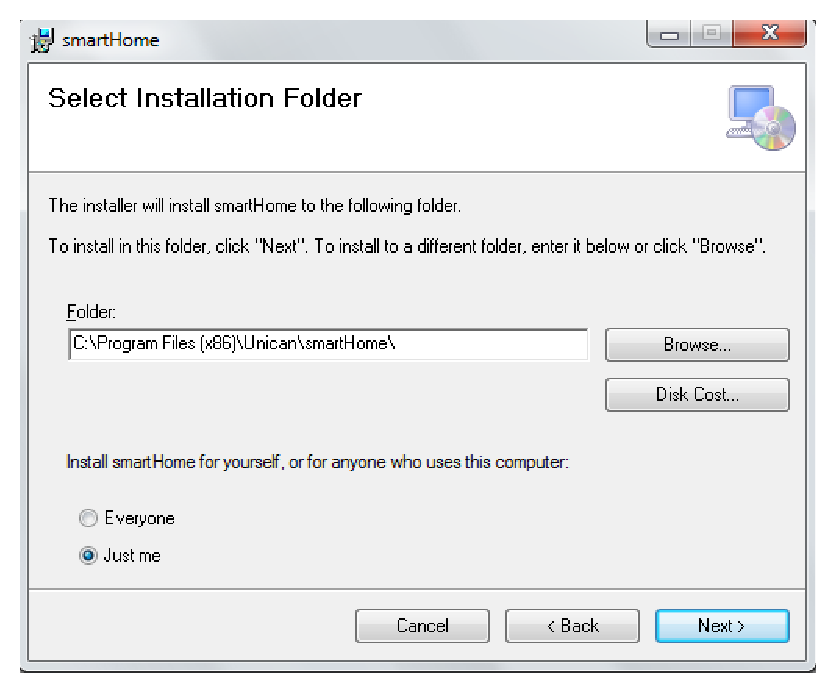
\includegraphics[width=.65\linewidth]{images/ubicacionModeller.eps}
            \vspace{1cm}
     \end{center}

\end{enumerate}

\subsection{Removing the plugin for the creation of models}
There are two ways to uninstall the plugin:
\begin{enumerate}
\item Come to our version of Windows to \emph{Control Panel}, then look for the option to uninstall programs and then discover our plugin by its name, \emph{SmartHome}.
\item If we have the installation file (\emph{SmartHomeModeller.msi}), open it and mark the option to uninstall(\emph{Remove SmartHome}).

     \begin{center}
            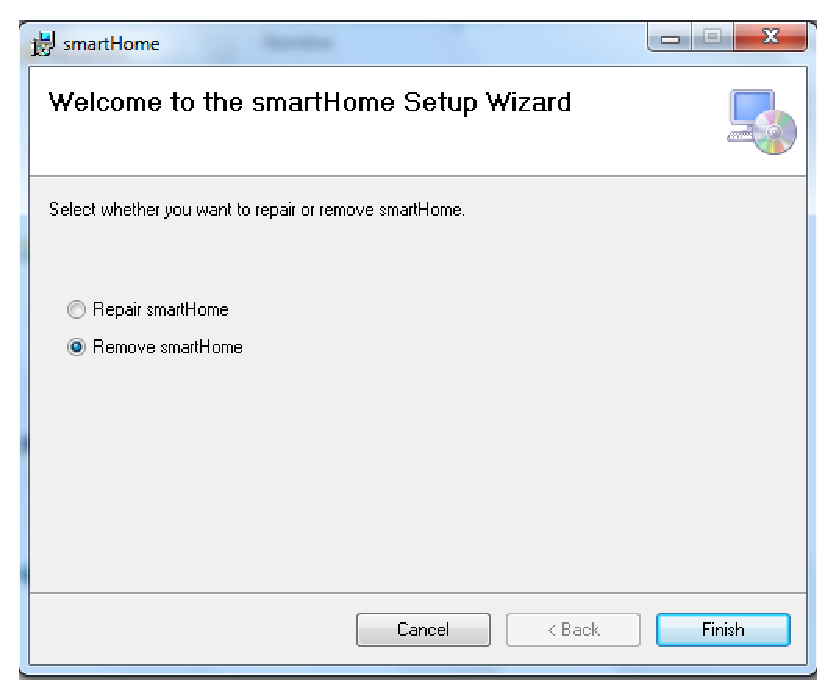
\includegraphics[width=.65\linewidth]{images/removeModeller.eps}
            \vspace{1cm}
     \end{center}
\end{enumerate}


\subsection{Installing the plugin that allows the creation of configurations}
 This plugin must be installed in the second place. To install, follow the next steps:

 \begin{enumerate}
 \item Go to the following URL:

    {\url{http://www.alumnos.unican.es/apr85/download}}

      and download the plugin \emph{smartHomeProject.vsix}.
 \item Go to the place where you downloaded the above file and double click on it.
 \item Follow the steps that appear in the wizard to complete the installation.

 \end{enumerate}


 \subsection{Removing the plugin that allows the creation of configurations}
 To uninstall this plugin must open Visual Studio 2010 and follow this steps:
 \begin{enumerate}
 \item Go to \emph{Tools} and select \emph{Extension Manager}.
    \begin{center}
            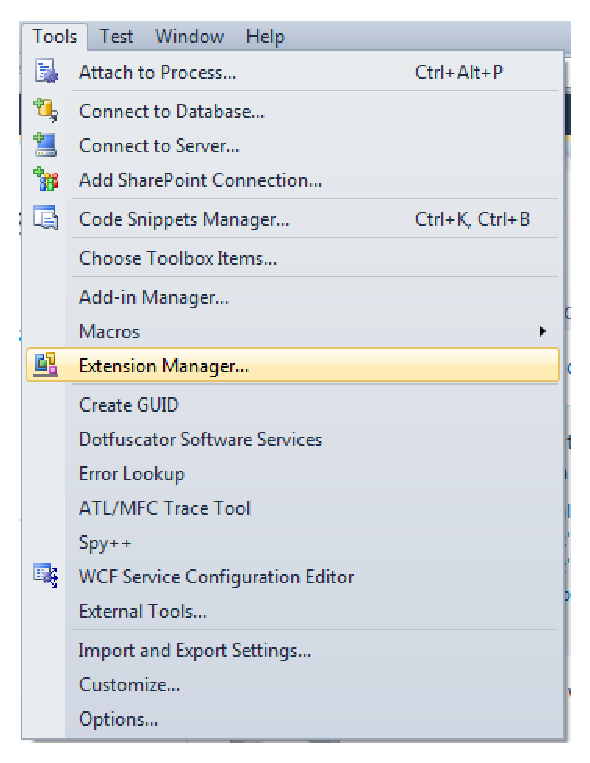
\includegraphics[width=.65\linewidth]{images/removeProject.eps}
            \vspace{1cm}
     \end{center}
 \item Select the extension, called \emph{Smart Home Project} and click on \emph{Uninstall}.

 \end{enumerate}

\section{Updates}
If there is a new version of one of the plugins in the web page \\(\url{http://www.alumnos.unican.es/apr85}),and you want to update, uninstall the current plugin and install the new version.
\end{document} 